\documentclass[11pt,a4paper
%,twocolumn
]{scrartcl}

% Support for UTF-8 and non-English letters require the following two
\usepackage[T1]{fontenc}
\usepackage[utf8]{inputenc}
% Font packages
\usepackage[default,defaultsans,oldstyle,proportional]{lato}
\usepackage[scaled]{beramono}
\usepackage{sfmath}
% Optimized justification via improved microtypography on character level
\usepackage{microtype}
\usepackage{ragged2e}
\usepackage[none]{hyphenat} % disable all hyphenation
\setlength{\emergencystretch}{3em} % allow extra hfill, needed if hyphenation disabled
%\overfullrule=1mm % mark overfull boxes
%\usepackage{showframe} % show edges of text areas
% Page layout
\usepackage[left=15mm,right=15mm,top=15mm,bottom=20mm,
   nohead,foot=10mm]{geometry}
% Page headers
\usepackage{scrlayer-scrpage}
\usepackage{lastpage}
% Page header
\KOMAoptions{headsepline=0pt,plainheadsepline=off}
\ihead*{}
\chead*{}
\ohead*{}
% Page footer
\KOMAoptions{footsepline=0pt,plainfootsepline=off}
\ifoot*{}
\cfoot*{Page \thepage{} of \pageref*{LastPage}}
\ofoot*{}
% Text layout
\KOMAoption{parskip}{never}
\newlength{\myparindent}
\newlength{\myparskip}
\setlength{\myparindent}{0pt}
\setlength{\myparskip}{5pt plus 1pt}
\setparsizes{\myparindent}{\myparskip}{0.1\linewidth plus 1fil}
\RedeclareSectionCommand[beforeskip=6pt,afterskip=3pt,afterindent=false]{section}
\RedeclareSectionCommand[beforeskip=6pt,afterskip=-0.5em,afterindent=false]{paragraph}
\RaggedRight
% SVN metadata
\usepackage[today,revrange,nofancy]{svninfo}
\svnInfo $Id$
% Graphics
\usepackage{graphicx}
% Colour definitions
\usepackage{xcolor}
\definecolor{secondary}{HTML}{435584}
% Floats
\usepackage{subcaption}
% Listings
\usepackage{listings}
\lstset{language=C, basicstyle=\small\ttfamily,
   aboveskip=0pt, belowskip=0pt}
\usepackage{upquote} % to use correct glyphs for single-quote in verbatim
% SI units
\usepackage{siunitx}
\sisetup{per-mode = symbol, detect-all = true}
% Hyperlinks
\usepackage[
   colorlinks=true,allcolors=secondary,breaklinks=true,
   bookmarks=true,unicode=true,bookmarksopen,bookmarksnumbered]{hyperref}
% Document-specific settings
\renewcommand\abstractname{Executive Summary}

% Document details
\title{Design Brief: Group 1}
\author{
   Kevin Costner,
   Sean Connery,
   Charles Martin Smith,
   Andy Garcia,
   Richard Bradford
   }
\date{\svnMaxToday, Document v.\svnInfoMaxRevision}

\begin{document}

\maketitle

\abstract{%
   Write an executive summary for your project. This should not overflow into
   the next page, should not contain references, and should be readable by
   a wide audience.
   }

\section{Introduction}
Write an introduction, explaining the purpose and background of this project.
Give a brief description of the game to be implemented.
References to be cited like so \cite{stroustrup2000}.
Also include an overview of this document.

\section{System Design}

\subsection{System overview}

The system will have two modes of operation, a mode for settings and 

\subsection{Software Modules}

The software modules proposed for the design are shown in Figure \ref{fig:software_components}. 

\begin{figure}
   \centering
   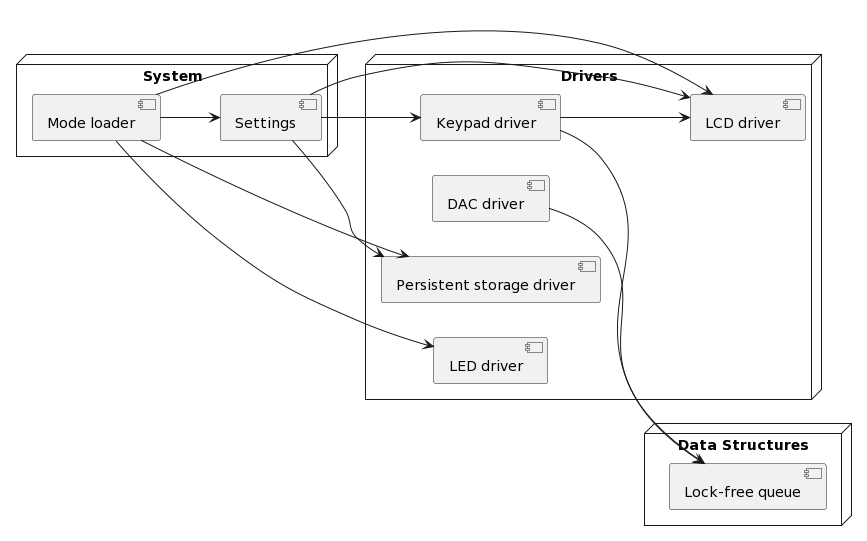
\includegraphics[width=0.9\textwidth]{software_components}
   \caption{Software components proposed for the system, grouped by functionality. Dashed arrows between components indicate dependencies.}
   \label{fig:software_components}
\end{figure}

Their responsibilities are as follows:

\begin{enumerate}
   \item Mode loader
      \begin{enumerate}
         \item Turn on the indicator LED (through the use of the LED driver).
         \item Present the user with options for choosing between settings mode, or normal mode (through the LCD driver).
         \item Process user's input (through the use of the button matrix driver).
         \item Load the system configuration from persistent storage if the normal mode is chosen (through the use of the persistent storage driver).
         \item Load code for the settings/normal mode depending on the user's choice.
      \end{enumerate}

   \item Settings
      \begin{enumerate}
         \item Present the user with options for configuring the system (through the use of the LCD driver).
         \item Process user's input (through the use of button matrix driver).
         \item Persist the system configuration (through the use of the persistent storage driver).
      \end{enumerate}

   \item Button matrix driver
      The behaviour of this component partially depends on the system's mode of operation.   
      \begin{enumerate}
         \item Polling cycle for the button matrix (this is used in all modes).
         \item Resets counter array.
         \item Displays buttons pressed on the LCD (this is used in normal mode).
         \item Pass buttons pressed via function-call return (this is used in the settings and entry modes).
         \item Keypad-driven interrupt handler logic (this is used in normal mode). Explained in a section below.
         \item Enable or disable the DAC driver.
      \end{enumerate}
   
   \item DAC driver
      Note that this component's code is meant to be encapsulated in a timer interrupt handler.
      This is the only way to reliably drive the DAC.
      The driver should have functionality allowing this handler to be disabled/enabled by the button matrix driver.
      \begin{enumerate}
         \item Read settings related to tone generation, and adapt accordingly.
         \item Keep track of a global counter in between handler invocations in order to track tone generation progress.
         \item Keep tones being generated in a global array that is NOT torn down between invocations of the timer interrupt.
         \item Produce DTMF tone when the timer interrupt is invoked.
      \end{enumerate}

   \item Persistent storage driver
      Note that this component is not as simple as it seems, since our microcontroller's flash memory will not have a filesystem.
      \begin{enumerate}
         \item Serialize and persist data to flash memory.
         \item Load and de-serialize data from flash memory.
      \end{enumerate}
   
   \item LED driver
      \begin{enumerate}
         \item Turn on LED on command.
         \item Turn off LED on comamnd.
      \end{enumerate}

   \item LCD driver
      \begin{enumerate}
         \item Encodes and displays an arbitrary C string on the LCD.
         \item Encodes and displays DTMF symbols on the LCD.
         \item Deals with automatic scrolling of displayed text.
      \end{enumerate}
\end{enumerate}

\subsection{Interaction between the button matrix driver and the DAC driver}

This interaction is particularly complex, and should be elucidated.

By default, the timer interrupt handler driving the DAC is disabled.

When a single invocation of the polling cycle detects one or more key presses, it performs the following operations:

\begin{enumerate}
   \item It immediately displays the symbols pressed on the LCD.
   \item It then pushes each symbol onto the lock-free queue in order of detection.
   \item It checks if there is a running timer interrupt. If not, it starts one.
   \item To start a timer interrupt, it determines the symbol's sampling frequency and loads the correct code. Resets global sample counter to 0.
\end{enumerate}

The timer interrupt handler does the following:

\begin{enumerate}
   \item Checks the global counter to see if it has to generate another tone sample.
   \item If yes, generates the tone. Increment the global sample counter.
   \item If no, checks the lock free queue. If this is not empty, it starts a new timer interrupt to generate the next tone.
\end{enumerate}

How do we deal with multiple tones being generated at the same time?

- If two tones have same base frequency, they interfere with each other.
- Even if not, they can still interfere as both are trying to drive the DAC, creating weird aliasing effects.

- If we use an output queue, how do we keep the system from getting out of sync with user's presses for long generation interval?
- Also, how do we trigger the next timer interrupt in the queue? Piggybacking on the interrupt handler (if counter reached end, enable next interrupt).

\subsection{Design phases}


\section{Management}
Include a time plan.
Show task dependencies.
How are these going to be managed?

\section{Closure}

\bibliographystyle{ieeetr}
\bibliography{references}

\end{document}
